\section{有限差分}
\label{sec:pdenum-finite-differences}

导数是极限，极限是算不完的，能算的是相邻几个值的差商。差商和导数差多少，由Taylor展开回答。

设$u$在$x$附近足够光滑。把$u(x\pm h)$在$x$处展开：
\[
 u(x\pm h)=u(x)\pm hu'(x)+\frac{h^2}{2}u''(x)\pm\frac{h^3}{6}u'''(x)+\frac{h^4}{24}u''''(\xi_\pm).
\]

只用一侧的值，得到前向差商和后向差商，它们与$u'(x)$相差$O(h)$。两式相减，偶次项消去，得到中心差商：
\begin{equation}
 \frac{u(x+h)-u(x-h)}{2h}=u'(x)+O(h^2).
 \label{eq:pdenum-central-first}
\end{equation}

两式相加，奇次项消去，得到二阶导数的三点公式：
\begin{equation}
 \delta_h^2u(x):=\frac{u(x-h)-2u(x)+u(x+h)}{h^2}=u''(x)+\frac{h^2}{12}u''''(\xi),
 \label{eq:pdenum-second-difference}
\end{equation}
其中$\xi\in(x-h,x+h)$，这里用到$u\in C^4$和介值定理，把两个余项合并成一个。

图~\ref{fig:pdenum-taylor-stencil}用$u=x^3$在$x=1$、$h=1/2$处比较三条割线。切线斜率是$3$，前向差商是$4.75$，后向差商是$1.75$，中心差商是$3.25$。两侧的偏差方向相反，取平均时一阶项抵消。

\begin{BookInlineFigure}
 \centering
 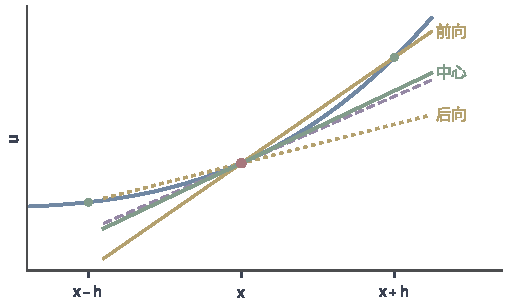
\includegraphics[width=86mm]{figures/06-differential-equations/02-partial-differential-equations/matplotlib/pdenum-taylor-stencil/figure.pdf}
 \caption{$u=x^3$（蓝）在红点$x=1$处的切线（紫色虚线）与三条差商割线，$h=1/2$。前向和后向差商（黄）分别偏大和偏小，中心差商（绿）的斜率$3.25$最接近切线的斜率$3$。}
 \label{fig:pdenum-taylor-stencil}
\end{BookInlineFigure}

余项里的$u''''$提醒我们：“二阶精度”不是公式本身的性质，而是公式加上解的光滑性的结论。解不够光滑时，式~\eqref{eq:pdenum-second-difference}的余项估计不成立，下面会看到实际阶数随之下降。

\subsection{椭圆方程的差分}
\label{sec:pdenum-elliptic-fd}

\paragraph{主要思想}
方程~\eqref{eq:pdenum-model}要求在每个内部节点$x_j$处成立，现在把它换成相邻三个节点值之间的关系。由式~\eqref{eq:pdenum-second-difference}，在$j=1,\ldots,n-1$上要求
\begin{equation}
 \frac{-U_{j-1}+2U_j-U_{j+1}}{h^2}=f(x_j),\qquad U_0=g_0,\quad U_n=g_1 .
 \label{eq:pdenum-three-point}
\end{equation}
这是$n-1$个未知量的线性方程组$\bm{A}_h\bm{U}=\bm{b}$。

边值出现在第一个和最后一个方程里。$j=1$的方程含已知的$U_0$，$j=n-1$的方程含已知的$U_n$，把它们移到右端，得到
\begin{equation}
 \bm{A}_h=\frac{1}{h^2}\begin{bmatrix}2&-1&&\\-1&2&\ddots&\\&\ddots&\ddots&-1\\&&-1&2\end{bmatrix},\qquad
 \bm{b}=\begin{bmatrix}f(x_1)+g_0/h^2\\f(x_2)\\\vdots\\f(x_{n-1})+g_1/h^2\end{bmatrix}.
 \label{eq:pdenum-fd-system}
\end{equation}

$\bm{A}_h$是三对角矩阵，按未知量的顺序消元时不产生新的非零元。一般的分解算法可参考\BookChapterRef{chap:direct-linear-solvers}{卷二第12章“线性方程的直接求解”}，这里只需要它的三对角形式。记对角元为$a_j$，上、下次对角元为$e_j$和$l_j$。消去第$j$行的下次对角元，逐行得到
\begin{equation}
 m_j=\frac{l_j}{d_{j-1}},\qquad d_j=a_j-m_je_{j-1},\qquad y_j=b_j-m_jy_{j-1}.
 \label{eq:pdenum-thomas-forward}
\end{equation}
消元后方程变成上双对角，再从最后一行往回代入：
\begin{equation}
 U_{n-1}=\frac{y_{n-1}}{d_{n-1}},\qquad U_j=\frac{y_j-e_jU_{j+1}}{d_j}.
 \label{eq:pdenum-thomas-back}
\end{equation}

\needspace{6\baselineskip}
\paragraph{变量}
\begin{itemize}
 \item $h=1/n$：步长；$x_j=jh$：节点，$j=0,\ldots,n$。
 \item $\bm{A}_h$：$(n-1)\times(n-1)$三对角矩阵，存为三个长度约$n$的数组。
 \item $\bm{b}\in\mathbb{R}^{n-1}$：节点上的右端，已含边值贡献。
 \item $d_j,y_j$：消元过程中的对角元和右端；$\bm{U}\in\mathbb{R}^{n-1}$：节点上的近似解。
\end{itemize}

\paragraph{初始化}
按式~\eqref{eq:pdenum-fd-system}填入$\bm{A}_h$与$\bm{b}$，并令$d_1=a_1$，$y_1=b_1$。

例中取$n=4$，$h=1/4$，$1/h^2=16$，$g_0=0$，$g_1=1$。节点上$f(x_j)=\pi^2\sin(\pi x_j)$，第三个方程的右端再加上$g_1/h^2=16$，于是
\[
 \bm{A}_h=16\begin{bmatrix}2&-1&0\\-1&2&-1\\0&-1&2\end{bmatrix},\qquad
 \bm{b}=\begin{bmatrix}6.9789\\9.8696\\22.9789\end{bmatrix}.
\]
初值是$d_1=32$，$y_1=6.9789$。

\needspace{6\baselineskip}
\paragraph{每轮更新}
对$j=2,\ldots,n-1$依次执行下面两步，第$n-1$行处理完后结束消元。
\begin{enumerate}
 \item 由式~\eqref{eq:pdenum-thomas-forward}算出$m_j,d_j$。例中第一轮$j=2$，第二轮$j=3$：
 \[
  \begin{aligned}
  m_2&=\frac{-16}{32}=-0.5, & d_2&=32-(-0.5)(-16)=24,\\
  m_3&=\frac{-16}{24}=-0.6667, & d_3&=32-(-0.6667)(-16)=21.3333.
  \end{aligned}
 \]
 \item 由同一式更新右端。例中两轮分别是
 \[
  \begin{aligned}
  y_2&=9.8696+0.5\times6.9789=13.3590,\\
  y_3&=22.9789+0.6667\times13.3590=31.8849.
  \end{aligned}
 \]
\end{enumerate}

消元结束后按式~\eqref{eq:pdenum-thomas-back}从下往上回代。例中依次得到
\[
 U_3=\frac{31.8849}{21.3333}=1.4946,\qquad
 U_2=\frac{13.3590+16\times1.4946}{24}=1.5530,
\]
\[
 U_1=\frac{6.9789+16\times1.5530}{32}=0.9946.
\]

最终得到节点上的近似解$(0.9946,\,1.5530,\,1.4946)$。式~\eqref{eq:pdenum-model-exact}给出的真值是$(0.9571,\,1.5000,\,1.4571)$，三个误差依次为$0.0375$、$0.0530$、$0.0375$。

\begin{BookInlineFigure}
 \centering
 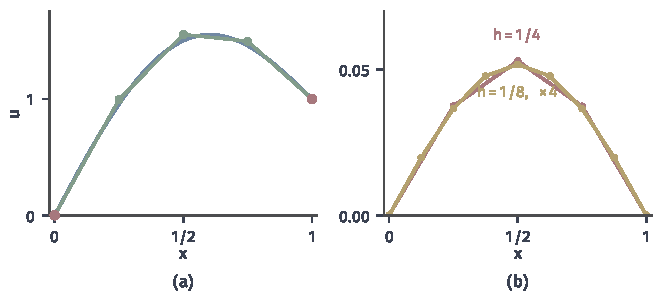
\includegraphics[width=112mm]{figures/06-differential-equations/02-partial-differential-equations/matplotlib/pdenum-fd-solution/figure.pdf}
 \caption{三点格式解问题~\eqref{eq:pdenum-model}。(a)$h=1/4$的数值解（绿）与真解（蓝），红点是边值。(b)节点误差，红线为$h=1/4$，黄线为$h=1/8$的误差乘以$4$：两条折线几乎重合，说明误差按$h^2$减小。}
 \label{fig:pdenum-fd-solution}
\end{BookInlineFigure}

图~\ref{fig:pdenum-fd-solution}(b)显示步长减半时误差约变为四分之一。这件事为什么成立？每个方程的残差很小，并不直接说明解的误差很小，下面要把两者联系起来。

\paragraph{从残差到误差}
把真解的节点值$\bm{R}_hu$代入离散方程，方程不再精确成立，差值就是\term{截断误差}（truncation error）：
\begin{equation}
 \bm{\tau}_h=\bm{A}_h\bm{R}_hu-\bm{b}.
 \label{eq:pdenum-truncation}
\end{equation}
由式~\eqref{eq:pdenum-second-difference}，$u\in C^4[0,1]$时它的每个分量满足$\lvert\tau_j\rvert\leq h^2M_4/12$，其中$M_4=\max\lvert u''''\rvert$。

离散解的误差$\bm{e}=\bm{R}_hu-\bm{U}$满足$\bm{A}_h\bm{e}=\bm{\tau}_h$，所以$\bm{e}=\bm{A}_h^{-1}\bm{\tau}_h$。问题归结为$\bm{A}_h^{-1}$的大小，而且这个大小不能随$h$变小而变大。这里要注意，$\bm{A}_h$的元素是$h^{-2}$量级，直接看它的元素说明不了逆的大小。

连续问题中，最大值原理控制了$-u''=f$的解（第~\ref{chap:elliptic-equations}章）。离散问题有完全平行的结论，证明也更短，因为“最大值点”只需在有限个数里找。

\begin{theorem}[离散最大值原理]
 \label{thm:pdenum-discrete-maximum}
 设网格函数$v_0,\ldots,v_n$在每个内部节点满足
 \begin{equation}
  \frac{-v_{j-1}+2v_j-v_{j+1}}{h^2}\leq0,\qquad j=1,\ldots,n-1,
  \label{eq:pdenum-discrete-subharmonic}
 \end{equation}
 则$\max_jv_j=\max(v_0,v_n)$。
\end{theorem}

\begin{proof}
 设最大值$M$在某个内部节点$j$取到。条件~\eqref{eq:pdenum-discrete-subharmonic}可以写成
 \[
  v_j\leq\frac{v_{j-1}+v_{j+1}}{2}.
 \]
 两个邻点都不超过$M$，而它们的平均不小于$v_j=M$，所以两个邻点都等于$M$。

 对邻点重复这个论证，最大值一路传到端点，于是$v_0=M$（也有$v_n=M$）。若最大值不在内部取到，它已经在端点上。
\end{proof}

这个定理的直观内容与热的抹平一致：每一点都不高于两邻点的平均，就不可能自己鼓起一个包。用它可以估计逆矩阵，诀窍是找一个差分算子作用后恰好等于$1$的函数。

\begin{theorem}[三点格式的误差界]
 \label{thm:pdenum-fd-error}
 对任意$\bm{\tau}\in\mathbb{R}^{n-1}$，$\bm{A}_h\bm{e}=\bm{\tau}$的解满足
 \begin{equation}
  \lVert\bm{e}\rVert_\infty\leq\frac18\lVert\bm{\tau}\rVert_\infty .
  \label{eq:pdenum-inverse-bound}
 \end{equation}
 若问题的解$u\in C^4[0,1]$，则
 \begin{equation}
  \max_j\lvert u(x_j)-U_j\rvert\leq\frac{h^2}{96}\max_{[0,1]}\lvert u''''\rvert .
  \label{eq:pdenum-fd-error}
 \end{equation}
\end{theorem}

\begin{proof}
 取$w(x)=x(1-x)/2$。它是二次函数，式~\eqref{eq:pdenum-second-difference}的余项为零，所以$-\delta_h^2w=-w''=1$，即$w$的节点值满足$\bm{A}_hw=\bm{1}$。

 令$v_j=e_j-\lVert\bm{\tau}\rVert_\infty w(x_j)$，并约定$e_0=e_n=0$。则$v_0=v_n=0$，且在内部节点上
 \[
  \frac{-v_{j-1}+2v_j-v_{j+1}}{h^2}=\tau_j-\lVert\bm{\tau}\rVert_\infty\leq0 .
 \]

 由定理~\ref{thm:pdenum-discrete-maximum}，$v_j\leq0$，即$e_j\leq\lVert\bm{\tau}\rVert_\infty w(x_j)$。对$-\bm{e}$作同样的论证，得到
 \[
  \lvert e_j\rvert\leq\lVert\bm{\tau}\rVert_\infty w(x_j) .
 \]

 $w$的最大值是$w(1/2)=1/8$，式~\eqref{eq:pdenum-inverse-bound}成立。把$\lVert\bm{\tau}_h\rVert_\infty\leq h^2M_4/12$代入，得到式~\eqref{eq:pdenum-fd-error}。
\end{proof}

证明的结构是后面反复出现的模式：一致性给出小的残差，稳定性（这里是$\lVert\bm{A}_h^{-1}\rVert_\infty\leq1/8$，常数与$h$无关）把残差转成解的误差。

例中$u''''=\pi^4\sin(\pi x)$，$M_4=\pi^4$，表~\ref{tab:pdenum-fd-refine}比较实际误差与上界。

\begin{BookInlineTable}
 \centering
 \caption{三点格式解问题~\eqref{eq:pdenum-model}的最大模误差和式~\eqref{eq:pdenum-fd-error}的上界。}
 \label{tab:pdenum-fd-refine}
 \begin{tabular}{cccc}
  \toprule
  $n$ & 实际误差 & 上界 & 相邻误差之比\\
  \midrule
  $4$ & $5.303\times10^{-2}$ & $6.342\times10^{-2}$ & --\\
  $8$ & $1.295\times10^{-2}$ & $1.585\times10^{-2}$ & $4.09$\\
  $16$ & $3.219\times10^{-3}$ & $3.964\times10^{-3}$ & $4.02$\\
  $32$ & $8.036\times10^{-4}$ & $9.909\times10^{-4}$ & $4.01$\\
  \bottomrule
 \end{tabular}
\end{BookInlineTable}

\paragraph{光滑性不够时}
误差界要求$u\in C^4$。换一个解$u=x^{3/2}-x$，它满足$u(0)=u(1)=0$，源项$f=-\tfrac34x^{-1/2}$在内部节点上有定义，但$u''$在$x=0$处无界，定理的条件不满足。

\begin{BookInlineFigure}
 \centering
 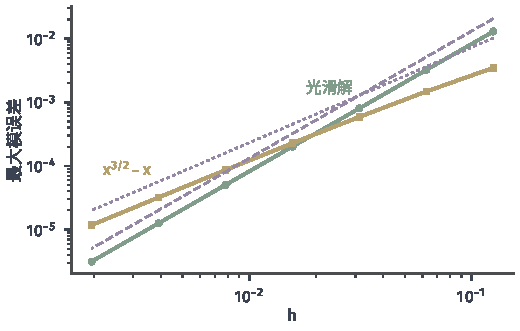
\includegraphics[width=88mm]{figures/06-differential-equations/02-partial-differential-equations/matplotlib/pdenum-fd-rates/figure.pdf}
 \caption{三点格式的网格加密，$n$从$8$到$512$，绿线是光滑解$\sin(\pi x)+x$，黄线是$x^{3/2}-x$。紫色虚线是斜率$2$，紫色点线是斜率$3/2$的参考线。公式没有改变，实际的收敛阶却取决于解的光滑性。}
 \label{fig:pdenum-fd-rates}
\end{BookInlineFigure}

图~\ref{fig:pdenum-fd-rates}是实际结果。光滑解每次加密的观测阶稳定在$2.00$附近。$x^{3/2}-x$的观测阶依次为$1.23$、$1.33$、$1.37$、$1.40$、$1.43$、$1.44$，逐渐向$3/2$靠近。这就是不能只凭公式形式判断精度的原因。

\paragraph{规则网格上的Poisson格式}
到两个空间维，在单位正方形上取步长$h$的规则网格。把$x_1$方向和$x_2$方向的三点公式相加，得到五点公式：
\begin{equation}
 \frac{4U_{i,j}-U_{i-1,j}-U_{i+1,j}-U_{i,j-1}-U_{i,j+1}}{h^2}=f(\bm{x}_{i,j}) .
 \label{eq:pdenum-five-point}
\end{equation}

边界上的节点值已知，出现时同样移到右端。图~\ref{fig:pdenum-five-point}(a)是模板的系数，(b)是$h=1/3$的网格，只有绿色的四个节点是未知量。

\begin{BookInlineFigure}
 \centering
 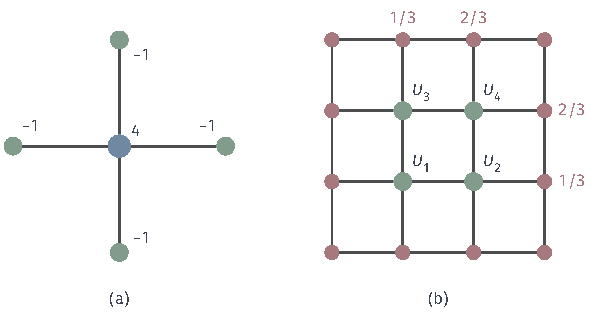
\includegraphics[width=101mm]{figures/06-differential-equations/02-partial-differential-equations/tikz/pdenum-five-point/figure.pdf}
 \caption{(a)五点模板，中心系数$4$，四个邻点系数$-1$，整体除以$h^2$。(b)$h=1/3$的网格，绿点是未知量，红点是已知的边值。边界标注是例子中边值$g=x_1x_2$在右边和上边的取值，左边和下边$g=0$。}
 \label{fig:pdenum-five-point}
\end{BookInlineFigure}

取$-\Delta u=0$，边值$g=x_1x_2$，真解就是$u=x_1x_2$。按图中编号，例如$U_2$的方程含右邻的边值$g(1,1/3)=1/3$，$U_4$的方程含右邻$g(1,2/3)$和上邻$g(2/3,1)$。乘以$h^2$并把边值移到右端，方程组是
\begin{equation}
 \begin{bmatrix}4&-1&-1&0\\-1&4&0&-1\\-1&0&4&-1\\0&-1&-1&4\end{bmatrix}
 \begin{bmatrix}U_1\\U_2\\U_3\\U_4\end{bmatrix}
 =\begin{bmatrix}0\\1/3\\1/3\\4/3\end{bmatrix}.
 \label{eq:pdenum-five-point-example}
\end{equation}

利用对称性$U_2=U_3$。第一个方程给出
\[
 U_2=2U_1 .
\]
代入第二个方程，得到
\[
 U_4=7U_1-\frac13 .
\]
最后一个方程成为$4U_4-2U_2=4/3$，代入上面两式，
\[
 24U_1=\frac83,\qquad U_1=\frac19,\quad U_2=U_3=\frac29,\quad U_4=\frac49 .
\]
这正是$x_1x_2$在四个节点上的值。原因是$x_1x_2$的四阶导数全为零，截断误差为零。

一般情形的误差估计与一维相同。设$u\in C^4(\overline{\Omega})$，比较函数仍取$w=x_1(1-x_1)/2$，它在五点算子下也给出$1$，所以$\lVert\bm{A}_h^{-1}\rVert_\infty\leq1/8$，最大模误差不超过$(h^2/96)(\max\lvert\partial_1^4u\rvert+\max\lvert\partial_2^4u\rvert)$。

矩阵的结构发生了变化。图~\ref{fig:pdenum-matrix-pattern}中，一维矩阵的非零元贴着对角线，二维矩阵除三条对角线外，还有两条离对角线一整行网格之远的带。按行消元时，带内的零元会被填满，所以二维问题的直接分解远比一维昂贵，第~\ref{sec:pdenum-error-cost}节再讨论这个代价。

\begin{BookInlineFigure}
 \centering
 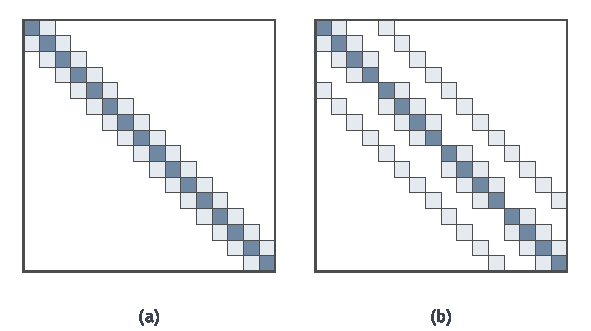
\includegraphics[width=100mm]{figures/06-differential-equations/02-partial-differential-equations/matplotlib/pdenum-matrix-pattern/figure.pdf}
 \caption{差分矩阵的非零元位置，深色是对角元。(a)一维三点格式，$16$个未知量。(b)二维五点格式，$4\times4$个内部节点，共$16$个未知量，按行编号。这里的方格本身是矩阵元素。}
 \label{fig:pdenum-matrix-pattern}
\end{BookInlineFigure}

规则网格的方便之处也是限制。边界不沿网格线时，靠近边界的节点需要专门的不等距模板，矩阵的对称性和最大值性质都要重新检查。下一节的有限元方法从弱形式出发，处理一般区域要自然得多。

\subsection{扩散方程的差分}
\label{sec:pdenum-heat-fd}

现在让温度随时间变化。考虑
\begin{equation}
 \partial_tu=\partial_x^2u\quad\text{于}\ (0,1)\times(0,T],\qquad u(0,t)=u(1,t)=0,\quad u(x,0)=u_0(x).
 \label{eq:pdenum-heat}
\end{equation}
这里只对空间做上一小节的离散，把时间留到下一步，这种做法称为\term{半离散}（semi-discretization）。

\paragraph{主要思想}
在内部节点上用三点公式代替$\partial_x^2u$，时间仍然连续，就得到常微分方程组
\begin{equation}
 \dot{\bm{U}}(t)=-\bm{A}_h\bm{U}(t),\qquad \bm{U}(0)=\bm{R}_hu_0 .
 \label{eq:pdenum-semidiscrete}
\end{equation}
偏微分方程变成了第~\ref{chap:ode-numerical-methods}章的线性系统，这正是把函数看成无限维向量所期待的对应：算子$\partial_x^2$对应矩阵$-\bm{A}_h$，它的特征模式对应矩阵的特征向量。

矩阵的特征向量恰好是正弦函数在节点上的取样。用三角恒等式
\[
 \sin(m\pi(j-1)h)+\sin(m\pi(j+1)h)=2\cos(m\pi h)\sin(m\pi jh)
\]
代入，得到$\bm{A}_h$的特征值
\begin{equation}
 \lambda_m=\frac{4}{h^2}\sin^2\frac{m\pi h}{2},\qquad m=1,\ldots,n-1 .
 \label{eq:pdenum-discrete-eigenvalues}
\end{equation}

$h\to0$时对固定的$m$有$\lambda_m\to m^2\pi^2$，这是连续算子的特征值。但$m$接近$n$时情形完全不同：最大特征值$\lambda_{n-1}=(4/h^2)\cos^2(\pi h/2)$接近$4/h^2$。

\begin{BookInlineFigure}
 \centering
 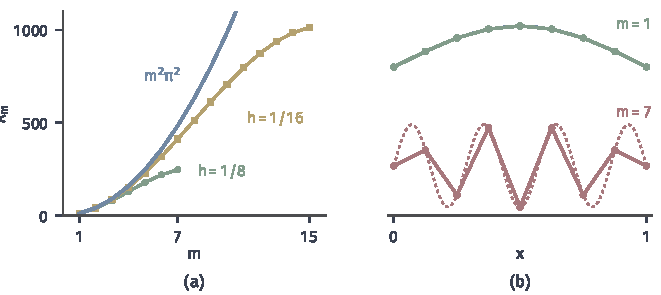
\includegraphics[width=112mm]{figures/06-differential-equations/02-partial-differential-equations/matplotlib/pdenum-heat-modes/figure.pdf}
 \caption{(a)连续特征值$m^2\pi^2$（蓝）与差分矩阵的特征值（绿$h=1/8$，黄$h=1/16$）。低模式贴近蓝线，高模式明显偏低，而网格越细，最大特征值越大。(b)$h=1/8$上的两个模式，绿线$m=1$，红线$m=7$；虚线是对应的连续正弦。}
 \label{fig:pdenum-heat-modes}
\end{BookInlineFigure}

图~\ref{fig:pdenum-heat-modes}说明了网格变细时发生的事。网格加密引入了越来越快的衰减模式，这些锯齿模式在真解中早已消失，也不是我们想算的东西，却决定了显式方法的步长上限。这与第~\ref{chap:ode-numerical-methods}章的刚性问题是同一件事。

在时间方向上，用步长$\tau$对式~\eqref{eq:pdenum-semidiscrete}作三种推进。三者的迭代公式为
\begin{align}
 \bm{U}^{(k+1)}&=(\bm{I}-\tau\bm{A}_h)\bm{U}^{(k)},
 \label{eq:pdenum-ftcs}\\
 \bm{U}^{(k+1)}&=(\bm{I}+\tau\bm{A}_h)^{-1}\bm{U}^{(k)},
 \label{eq:pdenum-btcs}\\
 \bm{U}^{(k+1)}&=\Bigl(\bm{I}+\frac{\tau}{2}\bm{A}_h\Bigr)^{-1}\Bigl(\bm{I}-\frac{\tau}{2}\bm{A}_h\Bigr)\bm{U}^{(k)}.
 \label{eq:pdenum-cn}
\end{align}
它们依次是显式Euler方法、后向Euler方法和\term{Crank--Nicolson方法}（Crank--Nicolson method）。第三种是梯形方法用在式~\eqref{eq:pdenum-semidiscrete}上的结果。

记$r=\tau/h^2$，式~\eqref{eq:pdenum-ftcs}的分量形式是
\begin{equation}
 U_j^{(k+1)}=U_j^{(k)}+r\bigl(U_{j-1}^{(k)}-2U_j^{(k)}+U_{j+1}^{(k)}\bigr).
 \label{eq:pdenum-ftcs-component}
\end{equation}

\needspace{6\baselineskip}
\paragraph{变量}
\begin{itemize}
 \item $\bm{U}^{(k)}\in\mathbb{R}^{n-1}$：第$k$层内部节点上的近似值。
 \item $h,\tau,r=\tau/h^2$：空间步、时间步及它们的比值。
 \item 后向Euler方法和Crank--Nicolson方法还要保存三对角矩阵及其消元结果$d_j$。
\end{itemize}

\paragraph{初始化}
令$U_j^{(0)}=u_0(x_j)$。例中取$h=1/4$，$u_0=\sin(\pi x)+0.1\sin(3\pi x)$，由它的两个模式可以写出真解：
\begin{equation}
 u(x,t)=\mathrm{e}^{-\pi^2t}\sin(\pi x)+0.1\,\mathrm{e}^{-9\pi^2t}\sin(3\pi x).
 \label{eq:pdenum-heat-exact}
\end{equation}
三个节点上的初值是
\[
 \bm{U}^{(0)}=(0.7778,\,0.9000,\,0.7778)^\top .
\]

\needspace{6\baselineskip}
\paragraph{每轮更新}
显式格式每轮按式~\eqref{eq:pdenum-ftcs-component}对$j=1,\ldots,n-1$算一遍，边界值$U_0=U_n=0$不更新，到$k\tau=T$结束。

例中先取$\tau=0.03$，$r=0.48$。第一轮中间节点的值是
\[
 U_2^{(1)}=0.9+0.48(0.7778-1.8+0.7778)=0.7827,
\]
左节点的值是
\[
 U_1^{(1)}=0.7778+0.48(0-1.5556+0.9)=0.4631 .
\]
此后各轮的结果为
\[
 \begin{aligned}
 \bm{U}^{(1)}&=(0.4631,\,0.7827,\,0.4631)^\top,\\
 \bm{U}^{(2)}&=(0.3942,\,0.4759,\,0.3942)^\top,\\
 \bm{U}^{(3)}&=(0.2442,\,0.3975,\,0.2442)^\top.
 \end{aligned}
\]
数值解有些摆动，但在衰减。把时间步改成$\tau=0.05$，$r=0.8$，前四轮是
\[
 \begin{aligned}
 \bm{U}^{(1)}&=(0.2533,\,0.7045,\,0.2533)^\top,\\
 \bm{U}^{(2)}&=(0.4116,\,-0.0174,\,0.4116)^\top,\\
 \bm{U}^{(3)}&=(-0.2609,\,0.6690,\,-0.2609)^\top,\\
 \bm{U}^{(4)}&=(0.6918,\,-0.8189,\,0.6918)^\top.
 \end{aligned}
\]
真解在$t=0.2$时中点的值是$0.1389$，而数值解已经变号并开始放大。

后向Euler方法每轮解一个三对角方程，用式~\eqref{eq:pdenum-thomas-forward}和式~\eqref{eq:pdenum-thomas-back}，矩阵的对角元是$1+2r$，次对角元是$-r$。例中$\tau=0.05$，$r=0.8$，第一轮的消元过程是
\[
 \begin{aligned}
 m_2&=-0.3077, & d_2&=2.3538, & y_2&=1.1393,\\
 m_3&=-0.3399, & d_3&=2.3281, & y_3&=1.1650,
 \end{aligned}
\]
从$d_1=2.6$和$y_1=0.7778$出发。回代给出
\[
 \bm{U}^{(1)}=(0.5004,\,0.6541,\,0.5004)^\top .
\]
第二、第三轮分别得到中点值$0.4565$和$0.3138$。同一个$\tau$下，Crank--Nicolson方法前三轮的中点值是$0.6358$、$0.3824$、$0.2391$，而真解是$0.6093$、$0.3727$、$0.2275$。它们都不放大。最终得到的是一列随时间衰减的向量，比较结果见下面对放大因子的分析。

\paragraph{放大因子解释一切}
对每个模式，$-\tau\lambda_m=z$，三种格式分别把这个模式乘上
\begin{equation}
 R_{\mathrm{E}}(z)=1+z,\qquad R_{\mathrm{B}}(z)=\frac{1}{1-z},\qquad R_{\mathrm{CN}}(z)=\frac{1+z/2}{1-z/2}.
 \label{eq:pdenum-heat-factors}
\end{equation}

例中$\lambda_1,\lambda_2,\lambda_3$分别约为$9.37$、$32$、$54.63$。$\tau=0.05$时，$R_{\mathrm{E}}$在三个模式上取$0.531$、$-0.6$、$-1.731$，第三个模式的绝对值大于$1$，放大的正是这个模式；$\tau=0.03$时，三个值是$0.719$、$0.04$、$-0.639$。图~\ref{fig:pdenum-amplification}把三条放大因子曲线和例中的点画在一起。

\begin{BookInlineFigure}
 \centering
 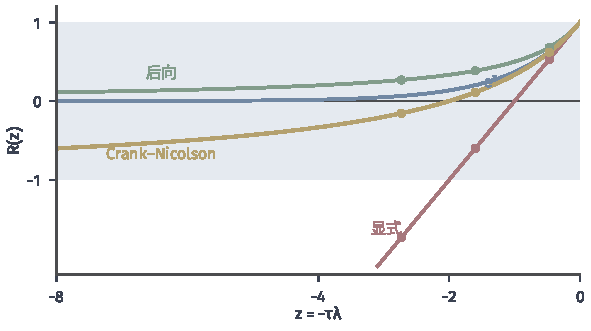
\includegraphics[width=100mm]{figures/06-differential-equations/02-partial-differential-equations/matplotlib/pdenum-amplification/figure.pdf}
 \caption{负实轴上的放大因子：蓝线是真解的$\mathrm{e}^{z}$，红线是显式Euler方法，绿线是后向Euler方法，黄线是Crank--Nicolson方法。浅蓝带表示$\lvert R\rvert\leq1$。圆点是$h=1/4$，$\tau=0.05$时三个模式的$z$值，显式Euler方法最左边的红点已在带外。}
 \label{fig:pdenum-amplification}
\end{BookInlineFigure}

显式格式要求所有模式都有$\lvert1+z\rvert\leq1$，即
\begin{equation}
 \tau\lambda_{\max}\leq2 .
 \label{eq:pdenum-ftcs-stability}
\end{equation}
由于$\lambda_{\max}<4/h^2$，$r=\tau/h^2\leq1/2$对任何网格都足够。例中$2/\lambda_{\max}=0.0366$，所以$\tau=0.03$稳定，$\tau=0.05$不稳定。

图~\ref{fig:pdenum-heat-stability}在$h=1/20$上比较阈值两侧。初值加了一个$2\times10^{-5}$大小的锯齿模式，它代表实际计算中总会出现的微小扰动。$r=0.55$时，这个几乎看不见的模式每步放大约$1.19$倍，到$t=0.08$时已经把解淹没。

\begin{BookInlineFigure}
 \centering
 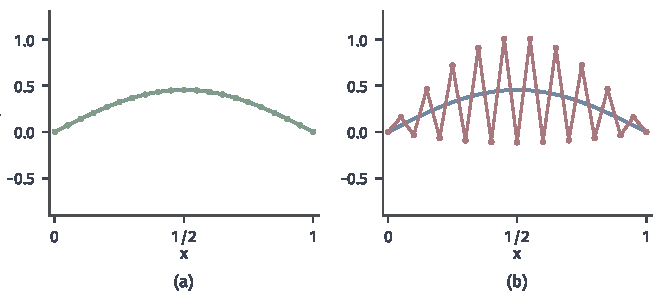
\includegraphics[width=112mm]{figures/06-differential-equations/02-partial-differential-equations/matplotlib/pdenum-heat-stability/figure.pdf}
 \caption{显式Euler方法在$h=1/20$上解式~\eqref{eq:pdenum-heat}到$t=0.08$，蓝线是真解。初值$\sin(\pi x)+0.1\sin(3\pi x)$叠加了幅度$2\times10^{-5}$的$\sin(19\pi x)$。(a)$r=0.4$，绿线贴合真解。(b)$r=0.55$，红线成为节点间振荡的锯齿。}
 \label{fig:pdenum-heat-stability}
\end{BookInlineFigure}

后向Euler方法对任何$z<0$都有$0<R_{\mathrm{B}}<1$，Crank--Nicolson方法也有$\lvert R_{\mathrm{CN}}\rvert<1$，它们都是无条件稳定的。但两者并不等价。$z\to-\infty$时，$R_{\mathrm{B}}\to0$，$R_{\mathrm{CN}}\to-1$，也就是说Crank--Nicolson方法几乎不衰减高模式，只是让它们每步变号。

\begin{BookInlineFigure}
 \centering
 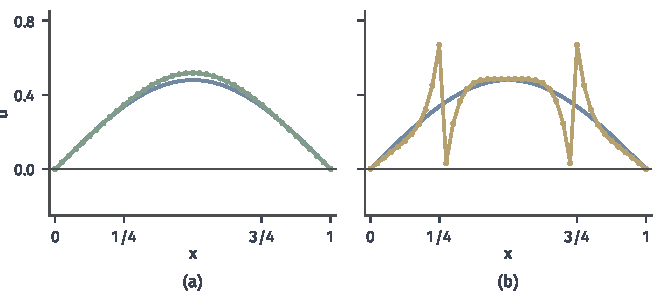
\includegraphics[width=112mm]{figures/06-differential-equations/02-partial-differential-equations/matplotlib/pdenum-cn-oscillation/figure.pdf}
 \caption{方波初值、$h=1/40$、$\tau=0.02$（$r=32$）走三步。蓝线是半离散系统的精确解。(a)后向Euler方法（绿）光滑，略有偏差。(b)Crank--Nicolson方法（黄）在间断附近保留了振荡，此时最高模式的放大因子约为$-0.97$。}
 \label{fig:pdenum-cn-oscillation}
\end{BookInlineFigure}

图~\ref{fig:pdenum-cn-oscillation}是这个差别的后果。初值的跳跃含有大量高模式，$r$很大时，Crank--Nicolson方法在跳跃处留下不衰减的尖峰，而真解在第一瞬间就把它们抹平了。“无条件稳定”只是说不放大，并不保证解的外观正确。

\paragraph{精度和稳定对步长的不同要求}
稳定性问的是误差会不会放大，精度问的是每步新引入多少误差。Taylor展开给出三种格式的截断误差：两种Euler方法是$O(\tau+h^2)$，Crank--Nicolson方法是$O(\tau^2+h^2)$。要让时间误差和空间误差平衡，所需的步长并不一样，表~\ref{tab:pdenum-heat-steps}汇总了这一点和实际的误差。

\begin{BookInlineTable}
 \centering
 \caption{热方程$u_0=\sin(\pi x)$到$T=0.1$的最大模误差。表头括号内是时间步的选取。}
 \label{tab:pdenum-heat-steps}
 \begin{tabular}{ccccc}
  \toprule
  $n$ & 显式（$r=0.4$） & 后向（$\tau=h$） & 后向（$\tau=h^2$） & CN（$\tau=h$）\\
  \midrule
  $10$ & $4.29\times10^{-3}$ & $1.33\times10^{-1}$ & $2.03\times10^{-2}$ & $2.99\times10^{-2}$\\
  $20$ & $1.06\times10^{-3}$ & $7.62\times10^{-2}$ & $5.24\times10^{-3}$ & $6.88\times10^{-3}$\\
  $40$ & $2.65\times10^{-4}$ & $4.14\times10^{-2}$ & $1.32\times10^{-3}$ & $1.69\times10^{-3}$\\
  $80$ & $6.62\times10^{-5}$ & $2.16\times10^{-2}$ & $3.31\times10^{-4}$ & $4.20\times10^{-4}$\\
  \bottomrule
 \end{tabular}
\end{BookInlineTable}

显式格式的$\tau\sim h^2$是稳定性强加的，时间精度因此多余。后向Euler方法稳定性上没有限制，但要达到$O(h^2)$，精度仍然要求$\tau\sim h^2$，表中$\tau=h$一列只有一阶收敛。Crank--Nicolson方法取$\tau\sim h$就够了，代价是对粗糙数据要小心。

二维和三维的规则网格上，$\lambda_{\max}$约为$4d/h^2$，显式稳定条件变成$r\leq1/(2d)$。同样地，这些稳定性结论都依赖矩阵的对称结构和这里的边界处理，第~\ref{sec:pdenum-stability}节回到这个问题。
